% !TeX root = ../../main.tex
\section{Results}\label{section:eval-results}

% Commands to edit stats which might change later. 

% demographic questions
\newcommand{\participantsCount}{23}
\newcommand{\participantsMale}{21}
\newcommand{\participantsAge}{23}

% model viewer statistical facts
\newcommand{\evalExpMvAvgPoses}{2.83}
\newcommand{\evalExpMvStdPoses}{1.94}
\newcommand{\evalExpMvParticipants}{\participantsCount}

% avg lp experiments
\newcommand{\kammAvgHits}{36.23/60}
\newcommand{\kammAvgStd}{6.87/60}
\newcommand{\youngAvgHits}{0.85}
\newcommand{\youngAvgStd}{-}
\newcommand{\oursAvgHits}{26.13/30}
\newcommand{\oursAvgStd}{5.52/30}

% model viewer sus scores
\newcommand{\evalExpMvSusScore}{83.04}
\newcommand{\evalExpMvSusGrade}{B}
\newcommand{\evalExpMvSusAdj}{\enquote{Good}}

% model viewer sus scores
\newcommand{\evalExpLpSusScore}{91.41}
\newcommand{\evalExpLpSusGrade}{A}
\newcommand{\evalExpLpSusAdj}{\enquote{Excellent}}

% model viewer sus scores
\newcommand{\evalExpVkSusScore}{71.63}
\newcommand{\evalExpVkSusGrade}{C}
\newcommand{\evalExpVkSusAdj}{\enquote{Ok}}

% Calculations
\newcommand{\participantsFemale}{\pgfmathparse{\participantsCount - \participantsMale}\pgfmathprintnumber[fixed, precision=2]{\pgfmathresult}}%chktex 8 chktex 1

%The results were evaluated in Python. Also, the plots were created using several Python libraries.

\participantsCount{} people participated in the evaluation. \participantsMale{} identified as male, the others identified as female. The average age is \participantsAge{} years. This could influence the results since younger people may have more exposure to new technologies and therefore, could pick up new technologies faster.
% The evaluation was conducted during different times of the day. does say nothing

The main disciplines and degrees of the participants are shown in Table~\ref{tab:sus-d}. As seen in Table~\ref{tab:sus-degree}, the highest degree of half of the participants is a high school degree or equivalent.
Table~\ref{tab:sus-discipline} exhibits that the disciplines are spread amongst different fields.

\begin{table}[H]
	\centering
	\begin{subtable}[b]{.48\textwidth}
		\footnotesize
		\centering
		\begin{tabular}[b]{l c c}
			\toprule
			Degree             & Count & Percentage \\
			\midrule
			High school degree & 13    & 56.52\%    \\
			Bachelor's degree  & 6     & 26.09\%    \\
			Master's degree    & 2     & 8.70\%     \\
			Diploma's degree   & 1     & 4.35\%     \\
			Approbation        & 1     & 4.35\%     \\
			\bottomrule
		\end{tabular}
		\caption{A table of the answers to Question A3: \enquote{What is the highest degree or level of school you have completed?} Most participants' (56.52\%) highest degree is the high school degree. Others (43.48\%) have at least one academic degree.}\label{tab:sus-degree}
  \end{subtable}%
  \hspace{0.04\textwidth}%
	\begin{subtable}[b]{.48\textwidth}
		\footnotesize
		\centering
		\begin{tabular}[b]{l c c}
			\toprule
			Discipline              & Count & Percentage \\
			\midrule
			Computer Science        & 7     & 30.43\%    \\
			Physics                 & 2     & 8.70\%     \\
			Automation and Robotics & 1     & 4.35\%     \\
			Book Science            & 1     & 4.35\%     \\
			Chemistry               & 1     & 4.35\%     \\
			Computational Biology   & 1     & 4.35\%     \\
			Economics               & 1     & 4.35\%     \\
			Electrical Engineering  & 1     & 4.35\%     \\
			Law                     & 1     & 4.35\%     \\
			Medicine                & 1     & 4.35\%     \\
			Musicology              & 1     & 4.35\%     \\
			Pharmacy                & 1     & 4.35\%     \\
			Public Service          & 1     & 4.35\%     \\
			Statistics              & 1     & 4.35\%     \\
			Technical Engineering   & 1     & 4.35\%     \\
			Technology Management   & 1     & 4.35\%     \\
			\bottomrule
		\end{tabular}
		\caption{A table of the answers to Question A4: \enquote{What is your main discipline?} Roughly one third (30.43\%) are computer science students. \participantsCount{} participants stated 16 different disciplines.}\label{tab:sus-discipline}
	\end{subtable}
	\caption[Degree and discipline of participants]{This table shows the participants' highest degree (Question A3) and main disciplines (Question A4).}\label{tab:sus-d}
\end{table}

All participants used their smartphone multiple times a day during the last six months. Most participants (78.26\%) used their computer to work or to study more than once per day during the last six months. 17.39\% state that they used it daily and only one participant used his or her computer one to three times a week for work or studies during the last six months.

As seen in Figure~\ref{fig:res-demo-q8-s3}, most participants (60.87\%) played computer games more than three times a month during the last six months. Figure~\ref{fig:res-demo-q8-s4} shows that most participants (91.30\%) used \gls{VR} less than once per month during the last six months. A huge portion (39.13\%) did not use \gls{VR} at all in the last six months.

\begin{figure}[H]
	\centering
	\begin{subfigure}[t]{.48\linewidth}%
		\centering
		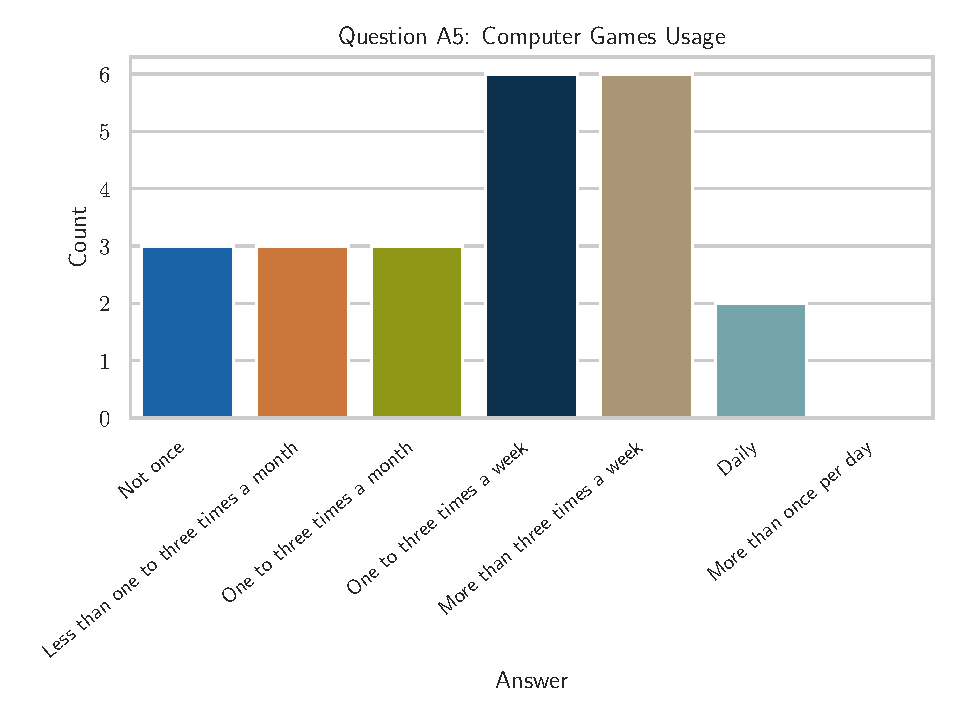
\includegraphics[width=\linewidth]{figures/evaluation/res_demo_q8_s3.pdf}
		\caption{The answers to the Question A5: \enquote{Please rate how much you used computer games in the last six months.}}\label{fig:res-demo-q8-s3}
	\end{subfigure}%
	\hspace{0.03\linewidth}
	\begin{subfigure}[t]{.48\linewidth}%
		\centering
		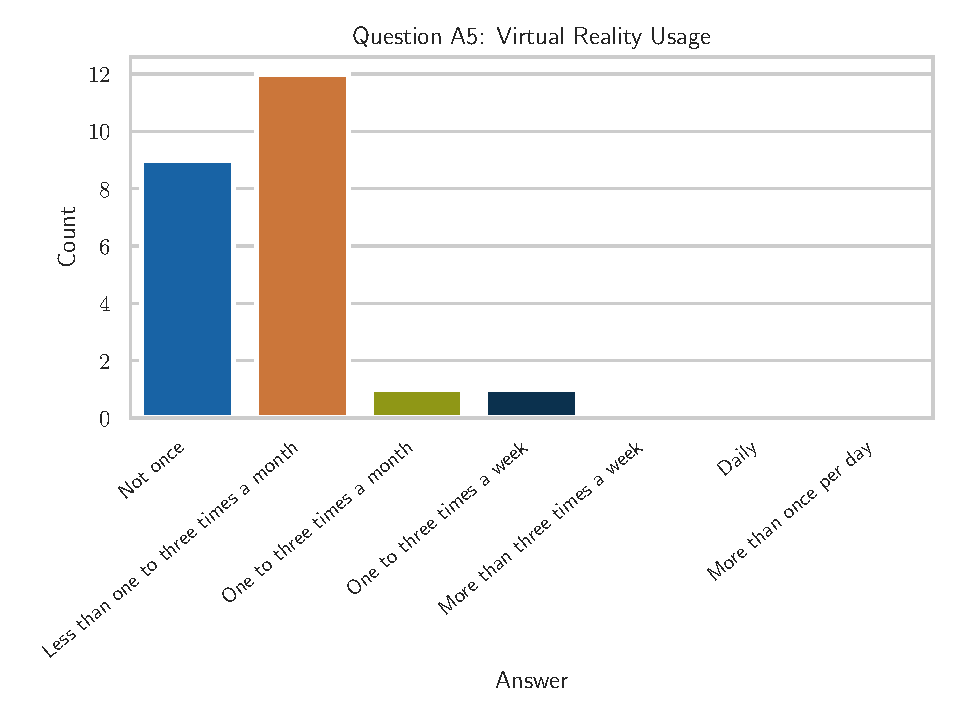
\includegraphics[width=\linewidth]{figures/evaluation/res_demo_q8_s4.pdf}
		\caption{The answers to the Question A5: \enquote{Please rate how much you used virtual reality headsets in the last six months.}}\label{fig:res-demo-q8-s4}
	\end{subfigure}%
	\caption[Computer games and VR usage]{The answers to the Question A5 about computer games and virtual reality usage. While \gls{VR} is used rarely, most survey participants (60.87\%) played computer games more than three times a month during the last six months. None of the participants is using \gls{VR} on a daily basis.}\label{fig:res-demo-q8}
\end{figure}

The participants were asked three questions regarding their experience with \gls{VR}, which could be answered with values ranging from one (\enquote{none}) to five (\enquote{a lot}). The first questions asked about the knowledge of the users about \gls{VR}. As can be seen in the box plots\footnote{The boxes indicate the range from the \nth{25} to the \nth{75} percentile. The bars outside the box (\enquote{whiskers}) indicate the \nth{90} and \nth{10} percentile. The median (\nth{50} percentile) is marked by the line in the center. Outliers are marked with diamond shapes.} in Figure~\ref{fig:res-demo-q9}, the general knowledge of \gls{VR} seems to be rather low (Mean: 2.83; \gls{STD}: 1.03).

\begin{figure}[H]
	\centering
	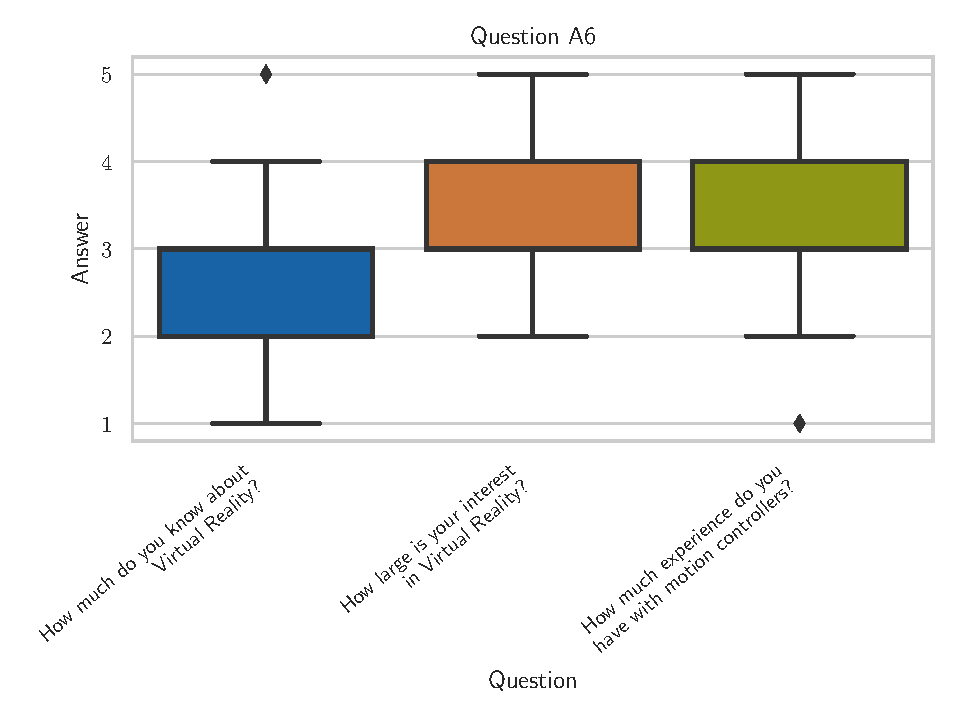
\includegraphics[width=10cm]{figures/evaluation/res_demo_q9.pdf}
	\caption[VR experience of the participants]{The answers to the Question A6 about the experience of the participants with \gls{VR}. The questions are rated with values ranging from one (\enquote{none}) to five (\enquote{a lot}). While the knowledge about \gls{VR} is rather low (Mean: 2.83; \gls{STD}: 1.03), the interest in the topic \gls{VR} is quite high (Mean: 3.48; \gls{STD}: 0.99). on average participants answered with 3.30 (\gls{STD}: 1.22) as an estimate for their experience with motion controllers.}\label{fig:res-demo-q9}
\end{figure}

The second question asked about the interest in \gls{VR} to which no participant answered with \enquote{none} (Mean: 3.48; \gls{STD}: 0.99). The last question asked about the experience with motion controllers. It was explicitly mentioned that the Wii remote counts as a motion controller, which might be the reason for the high average being above the one asking about the knowledge of \gls{VR} (Mean: 3.30; \gls{STD}: 1.22).


\subsection{Model Viewer}\label{section:eval-res-mv}

The model viewer experiment (described in Section~\ref{section:model-viewer}) allows users to view a three-dimensional model from different angles. To benchmark extensive usage, the users had to match the orientation of the model with the orientation of a second model instance in a golden color (the target). After starting the task, the target is spawned with a random orientation.
Since in the current implementation, the model cannot be rotated upside down (as mentioned in Section~\ref{subsection:topic-data}), only reachable target positions are generated.

As soon as the task is started, users have 30 seconds to match as many orientations as possible. Similar to the implementation by \citeauthor{Katzakis.2010} (presented in Section~\ref{section:katzakis-2010}), the target is rotated to a new random orientation after one orientation was matched~\cite[140]{Katzakis.2010}.
Because it is hard to match the rotation exactly on all three axes, it is sufficient to pose the model in a similar orientation to the target. A similar pose is reached when the smallest angle between the two rotations is less than 20 degrees.

%  T-Test:
%\pgfmathparse{(\evalExpMvAvgPoses-6.5)/(\evalExpMvStdPoses/sqrt(\evalExpMvParticipants))}\pgfmathprintnumber[fixed, precision=2]{\pgfmathresult} 
% chktex 1
\citeauthor{Katzakis.2010} tracked the time it takes to match a pre-defined pose with a smartphone, a mouse, and a touch panel. The lowest time on average to match one pose, 6.5 seconds, was achieved using the smartphone as an input device~\cite[140]{Katzakis.2010}. As seen in Figure~\ref{fig:eval-exp-mv}, the average time it took to match a correct pose in the model viewer experiment presented in this thesis is roughly \evalExpMvAvgPoses{} seconds, which is lower than the average time of \citeauthor{Katzakis.2010}. This can be due to the fact that users never had to turn the smartphone entirely upside down, because of the previously mentioned limitation.

\begin{figure}[H]
	\centering
	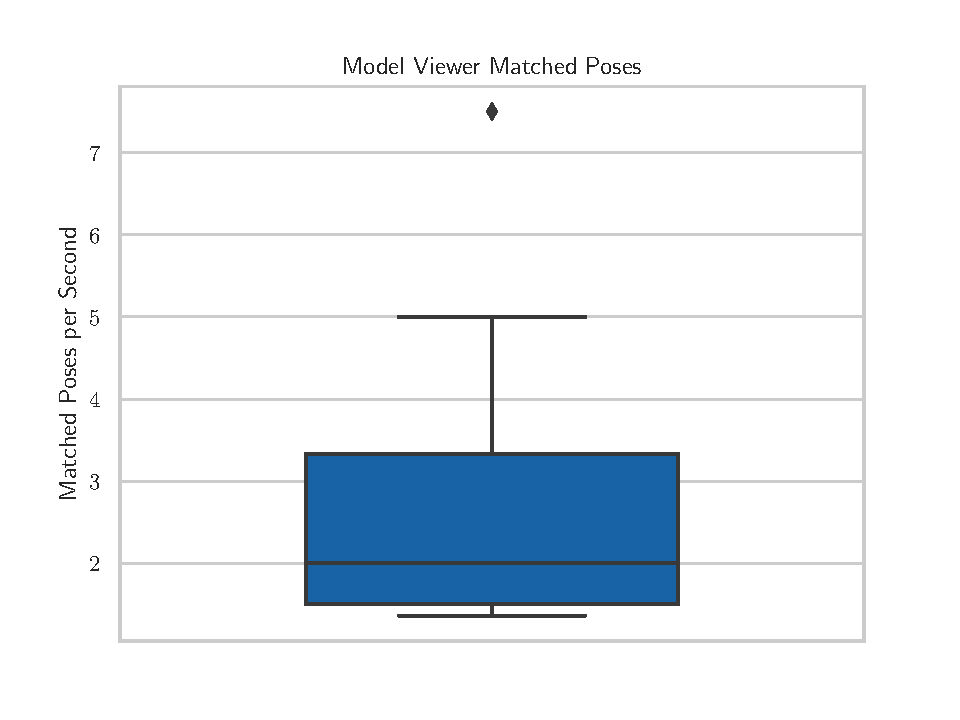
\includegraphics[width=10cm]{figures/evaluation/eval_exp_mv.pdf}
	\caption[Model viewer task results]{The time in seconds it took to match a correct pose in the model viewer experiment.}\label{fig:eval-exp-mv}
\end{figure}

Another reason for the lower average time is that the target and the controlled model are not displayed in two separate locations like in {\citetitle{Katzakis.2010}} by \citeauthor{Katzakis.2010}, but instead with the same origin in the same coordinate space, which makes it easier to see the difference between both rotations~\cite[140]{Katzakis.2010}. Also, the fact that a skeleton model, instead of a multi-colored cube was used, could play a role.

Not only the measured statistics from the experiment but also the \gls{SUS} study results indicate a useable implementation, as seen in Figure~\ref{fig:exp-mv-stats}. A score of \evalExpMvSusScore{} is considered \evalExpMvSusAdj{} and mapped to grade \evalExpMvSusGrade, according to \citeauthor{Bangor.2009}~\cite[120\psq]{Bangor.2009}.

\begin{figure}[H]
	\centering
	\begin{subfigure}[t]{.48\linewidth}%
		\centering
		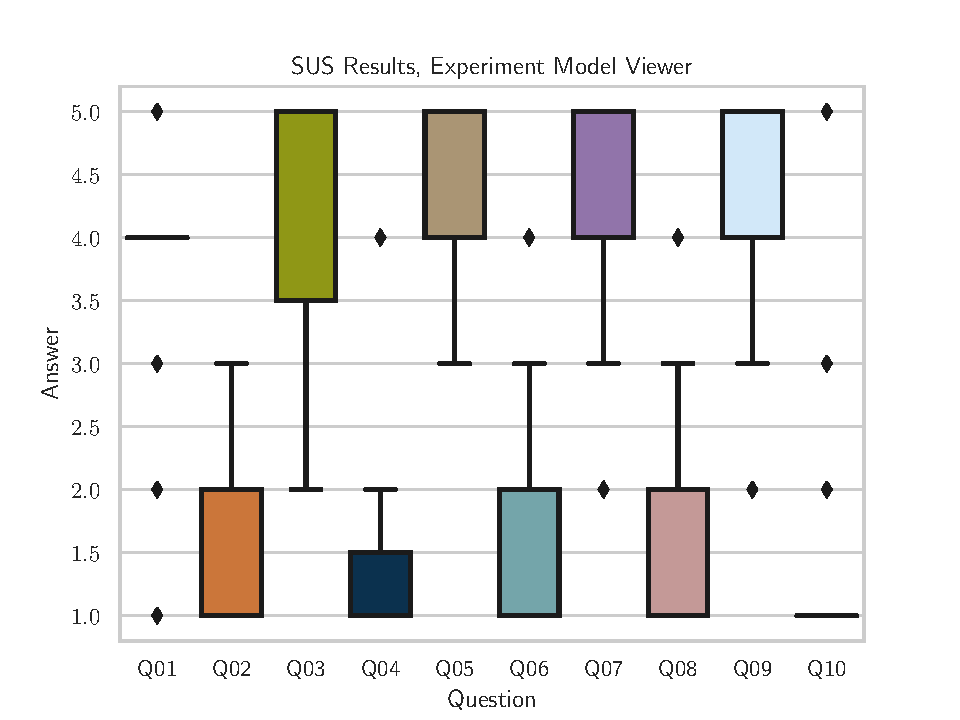
\includegraphics[width=\linewidth]{figures/evaluation/res_exp_mv.pdf}
		\caption{The results of questions one to ten.}\label{fig:res-exp-mv}
	\end{subfigure}%
	\hspace{0.03\linewidth}%
	\begin{subfigure}[t]{.48\linewidth}%
		\centering
		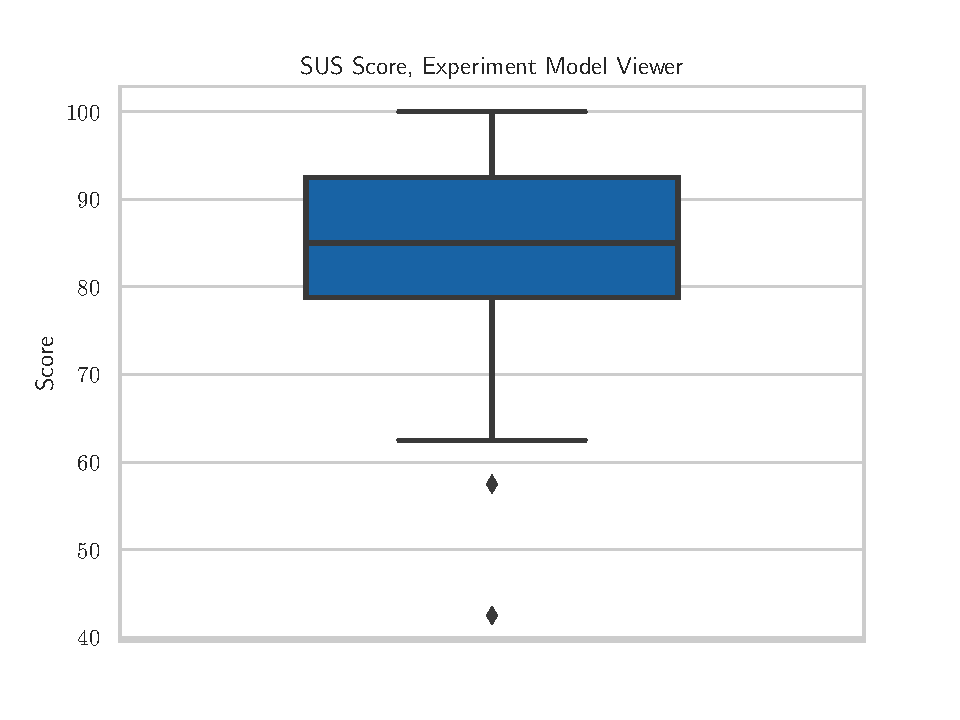
\includegraphics[width=\linewidth]{figures/evaluation/score_exp_mv.pdf}
		\caption{The overall \gls{SUS} score.}\label{fig:score-exp-mv}
	\end{subfigure}%
	\caption[Model viewer SUS results]{The results of the \gls{SUS} user study for the model viewer.}\label{fig:exp-mv-stats}
\end{figure}

Participants provided additional feedback after the \gls{SUS} user study. They raised the concern that the phone is too large and has a weird shape for controlling a three-dimensional model on the display. Since every device with basic web capabilities and sensors similar to a smartphone could be used, it would be no problem to use another more comfortable device. 


\subsection{Laser Pointer}\label{section:eval-res-lp}

Section~\ref{section:laser-pointer} introduces the laser pointer experiment. To test the performance of participants using this interaction, the participants had to select as many targets as possible in 30 seconds. The users were told to be as fast and in particular as accurate as possible since the miss-hits are counted. To trigger a selection, the users have to touch the smartphone display, which counts as one click. If no target was selected, a miss is counted. The total selection (click) count is the sum of hits and miss-clicks.

%Cubes were chosen as target objects, because \gls{UI} elements are often rectangular like the two-dimensional projection of a cube.
Three cubes (the targets) are spawned at random locations in front of the users. The cubes are always spawned in the view of the users so that the users do not have to look for the targets actively. 
If one cube was hit, another one is spawned, so that three cubes are always visible. This is important because the users can plan to hit the next target while aiming for the current one. Otherwise, the task would test the users' reaction time, which is not desired. It was found that three cubes are a good amount because too many targets would clutter not only the view but also shorten the aiming periods.

Figure~\ref{fig:eval-exp-lp} visualizes the total click count (Mean: 31.83; \gls{STD}: 6.89), the actual hit count (Mean: 26.13; \gls{STD}: 5.52) and the count of miss-hits (Mean: 5.70; \gls{STD}: 4.37) per 30 seconds. Participants were able to successfully point to and select objects with a speed of nearly one click per second. As seen in Figure~\ref{fig:eval-exp-lp-ratio-scatter}, the hit to miss ratio is very high for slightly lower speeds but decreases quickly with higher click speeds.

\begin{figure}[H]
	\centering
	\begin{subfigure}[t]{.48\linewidth}%
		\centering
		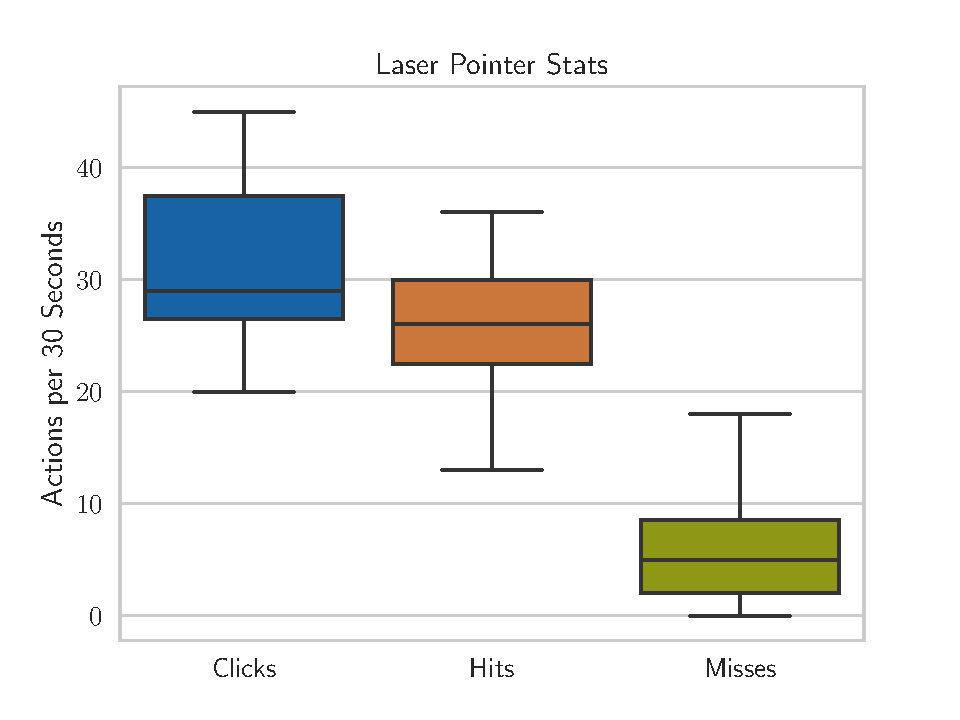
\includegraphics[width=\linewidth]{figures/evaluation/eval_exp_lp.pdf}
		\caption{The count of clicks, hits and misses per 30 seconds. Clicks are the sum of hits and misses.}\label{fig:eval-exp-lp}
	\end{subfigure}%
	\hspace{0.02\linewidth}%
	\begin{subfigure}[t]{.48\linewidth}%
		\centering
		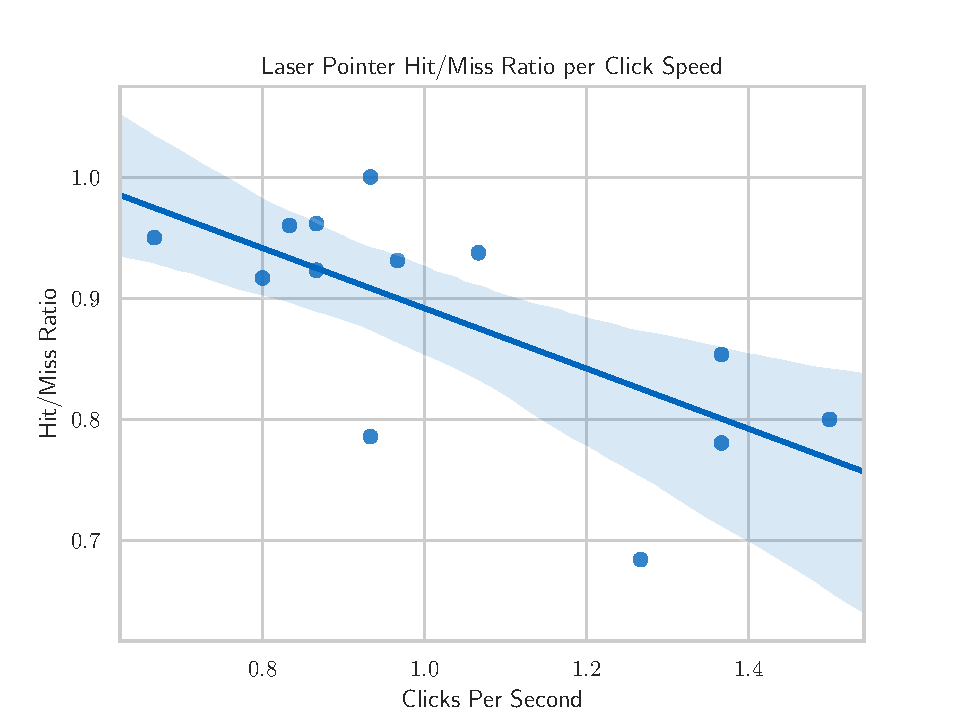
\includegraphics[width=\linewidth]{figures/evaluation/eval_exp_lp_ratio_scatter.pdf}
		\caption{The hit to miss ratio per click speed.}\label{fig:eval-exp-lp-ratio-scatter} %The line visualizes the linear regression with a 95\% confidence interval.
	\end{subfigure}%
	\caption[Laser pointer task results]{These figures represent the measured statistics of the laser pointer experiment. Participants hit targets more often (Mean: 26.13; \gls{STD}: 5.52) than they missed targets (Mean: 5.70; \gls{STD}: 4.37) on average per 30 seconds. The hit to miss ratio decreases with increasing click speeds.}\label{fig:exp-lp-eval}
\end{figure}

The performance of this experiment is hard to compare with other implementations without a standardized experiment setup. For example, the size, shape, position, and distance of the targets as well as the spawn area and whether distracting elements are present, varies between different task evaluations of other research. However, a comparison should still give a rough estimate of the performance. Often the hit count is measured in different time intervals. To compare the results, the average hit count per second is calculated.

\citeauthor{Kamm.2018} tested his implementation in a similar \gls{VR} scenario with a wrist band as an input device. To compare his implementation, he also tested a laser pointer approach using a \gls{VR} motion controller~\cite[39]{Kamm.2018}. A significant difference in his experiment setup is that only one target is displayed at a time. Another difference is that users have to rotate their head more in order to see the targets as they are placed in a 90-degree radius. An arrow, which always points to the next target, is displayed to prevent wasting time while searching for the next target. Also, the distance from the users to the targets is randomized~\cite[45]{Kamm.2018}.

\citeauthor{JiYoungOh.2002} compared a real-world laser pointer for large screen interactions to a computer mouse. The application is displayed through a projector, and the laser is detected by a camera. The pointer-device also has a button, which is pressed down to select an object, similar to the laser pointer implementation presented in Section~\ref{section:eval-res-lp}. All targets are always visible and have to be selected in a pre-determined order. Also, the fact that all objects are on the same plane makes the task similar to the one presented in this thesis~\cite[3\psq]{JiYoungOh.2002}.

As seen in Table~\ref{tab:lp-comp}, the technique presented in Section~\ref{section:eval-res-lp} is the one with the best results. However, due to the different conditions and task setups, it is not possible to draw a strong conclusion. Still, the result is similar to a real-world pointing technique, which suggests good usability.

\begin{table}[H]
	\centering
	\begin{tabular}{l c c}
		\toprule
		Source                                            & Average Hits per Second                                                            & Standard Deviation                                                                \\
		\midrule
		\citeauthor{Kamm.2018}~\cite{Kamm.2018}           & \pgfmathparse{\kammAvgHits}\pgfmathprintnumber[fixed, precision=2]{\pgfmathresult} & \pgfmathparse{\kammAvgStd}\pgfmathprintnumber[fixed, precision=2]{\pgfmathresult} \\%chktex 2
		\citeauthor{JiYoungOh.2002}~\cite{JiYoungOh.2002} & \(\youngAvgHits{}\)                                                                  & \(\youngAvgStd{}\)                                                                  \\%chktex 2 21
		Section~\ref{section:eval-res-lp}                 & \pgfmathparse{\oursAvgHits}\pgfmathprintnumber[fixed, precision=2]{\pgfmathresult} & \pgfmathparse{\oursAvgStd}\pgfmathprintnumber[fixed, precision=2]{\pgfmathresult} \\
		\bottomrule
	\end{tabular}
	\caption[Comparison of laser pointer task results]{This table compares the average hits per second from similar laser pointer evaluations of other research. The implementation from Section~\ref{section:eval-res-lp} achieved the highest average hits per second.}\label{tab:lp-comp}
\end{table}

Not only the measured interaction times but also the \gls{SUS} study results indicate a useable implementation, as seen in Figure~\ref{fig:exp-lp-stats}. A score of \evalExpLpSusScore{} is considered \evalExpLpSusAdj{} and mapped to grade \evalExpLpSusGrade{}, according to \citeauthor{Bangor.2009}~\cite[120\psq]{Bangor.2009}.

\begin{figure}[H]
	\centering
	\begin{subfigure}[t]{.48\linewidth}%
		\centering
		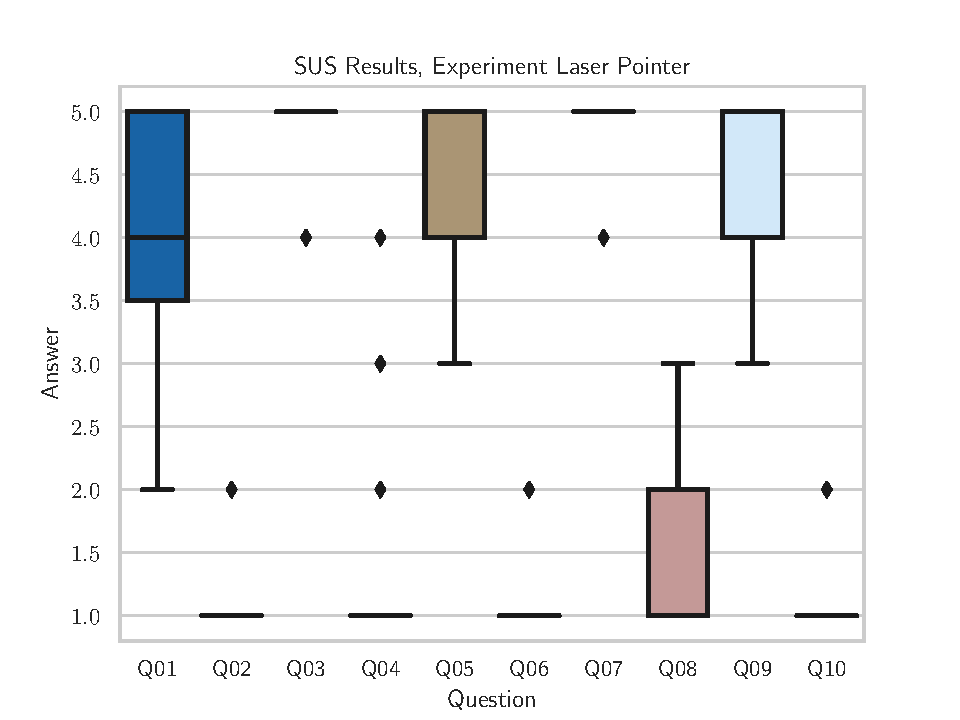
\includegraphics[width=\linewidth]{figures/evaluation/res_exp_lp.pdf}
    \caption{The results of questions one to ten.}\label{fig:res-exp-lp}
	\end{subfigure}%
	\hspace{0.04\linewidth}%
	\begin{subfigure}[t]{.48\linewidth}%
		\centering
		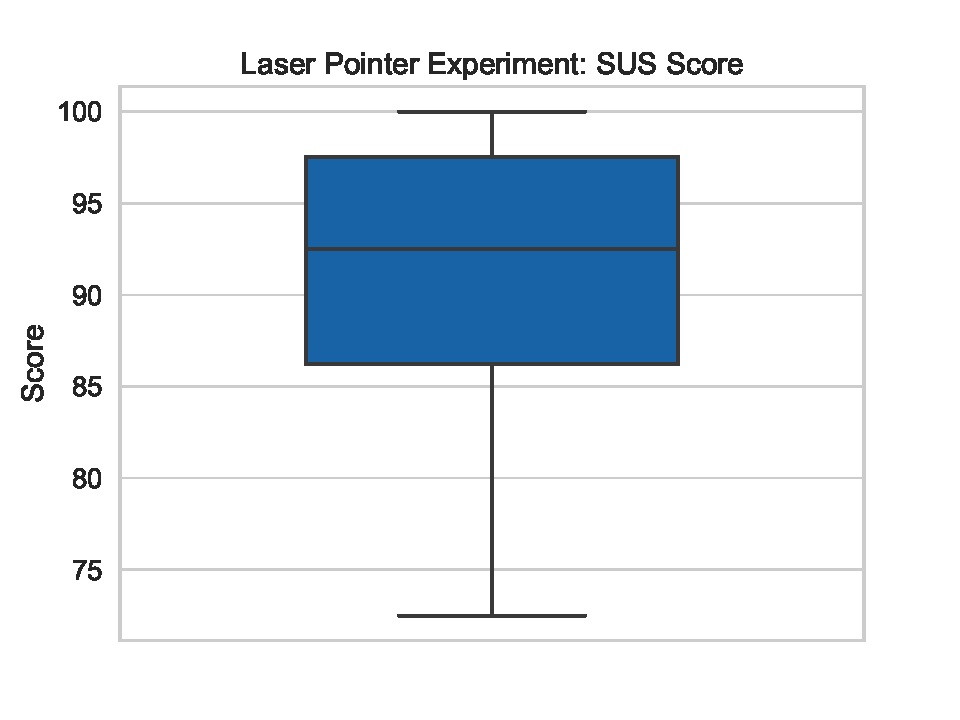
\includegraphics[width=\linewidth]{figures/evaluation/score_exp_lp.pdf}
		\caption{The overall \gls{SUS} score.}\label{fig:score-exp-lp}
	\end{subfigure}%
	\caption[Laser pointer SUS results]{The results of the \gls{SUS} user study for the laser pointer. Ignoring a few outliers, participants clearly agree on most \gls{SUS} questions, as seen in Figure~\ref{fig:res-exp-lp}.}\label{fig:exp-lp-stats}
\end{figure}

Some participants mentioned that it is hard to notice whether the laser pointer is hitting an object or not. They suggested better indicators, like a bigger laser beam or an indicator at the position where the laser hits an object.


\subsection{Virtual Keyboard}\label{section:eval-res-vk}

The task for the virtual keyboard experiment (presented in Section~\ref{section:virtual-keyboard}) is to enter a text as fast as possible without mistakes. The text chosen for this task is \enquote{A quick brown fox jumps over the lazy dog}, which is commonly used when testing keyboards, typewriters or fonts because it contains every character of the alphabet.

To test special characters, an exclamation mark is also added to the end of the task's text. This given text is displayed above the text, which is being typed using the keyboard. If a mistake was made, it has to be corrected in order to complete the task. After starting the task, a timer counts the time until the \enquote{enter}-button is pressed.

The number of corrections the participants made while entering the given text has an average of 2.7 corrections (mean: 2.74; \gls{STD}: 2.38). A correction is counted when users used the \enquote{backspace}-key to remove one character. If the participants did not recognize their error soon enough, it is possible that in order to correct one letter, they had to remove multiple characters, because it is not possible to move the caret. Since participants had to type a total of 42 characters, the average correction count to character count ratio is at 6.52\%.
Participants took 31.7 seconds on average (\gls{STD}: 5.1) to complete the task. Figure~\ref{fig:eval-exp-vk-ratio-scatter} shows that the more mistakes were made, the more time users needed to complete the task.
%Since the word count of the sentence, the users have to type in the task is 9 and the average time to type those is 31.7 seconds, the typing speed can be estimated using the rule of three with 17 words per minute (\(60*9/31.7\)). To measure the typing speed % wrong calculation of wpm

\begin{figure}[H]
	\centering
	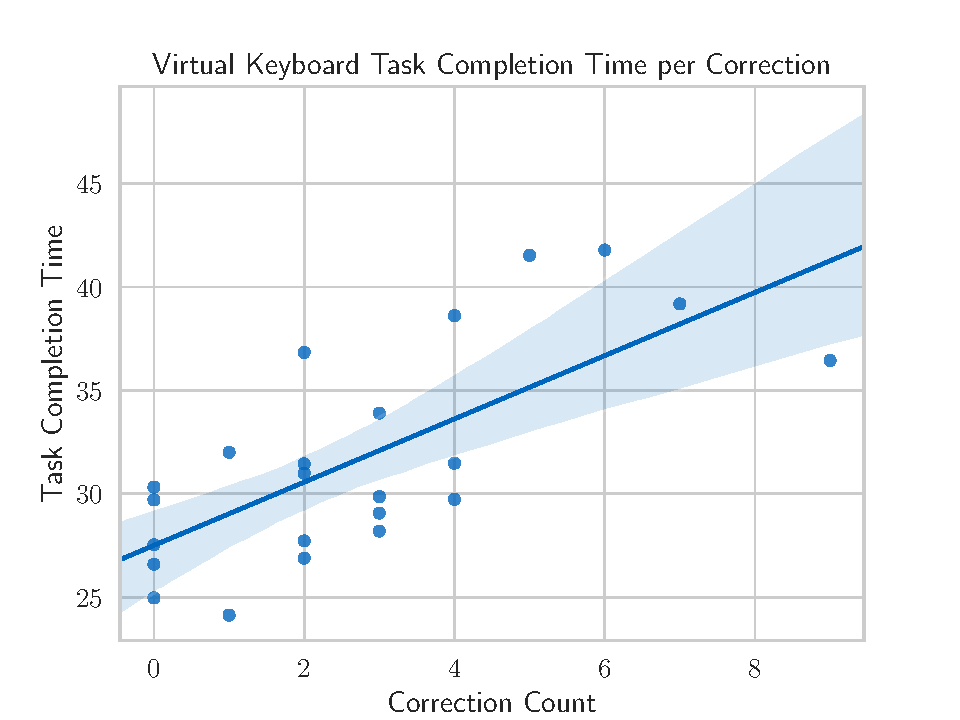
\includegraphics[width=10cm]{figures/evaluation/eval_exp_vk_ratio_scatter.pdf}
	\caption[Virtual keyboard task results]{A scatter plot of the time it took to complete the virtual keyboard task per correction count. The line visualizes the linear regression with a 95\% confidence interval. The more corrections were made, the longer participants took to complete the task.}\label{fig:eval-exp-vk-ratio-scatter}
\end{figure}

The \gls{SUS} score for this experiment, shown in Figure~\ref{fig:exp-mv-stats}, is \evalExpVkSusScore{}.
According to \citeauthor{Bangor.2009}, this score is considered \evalExpVkSusAdj{} and mapped to grade \evalExpVkSusGrade~\cite[120\psq]{Bangor.2009}. Since this score is still in the \enquote{acceptable} range~\cite[120\psq]{Bangor.2009}, it can be considered \enquote{usable}.

\begin{figure}[H]
	\centering
	\begin{subfigure}[t]{.5\linewidth}%
		\centering
		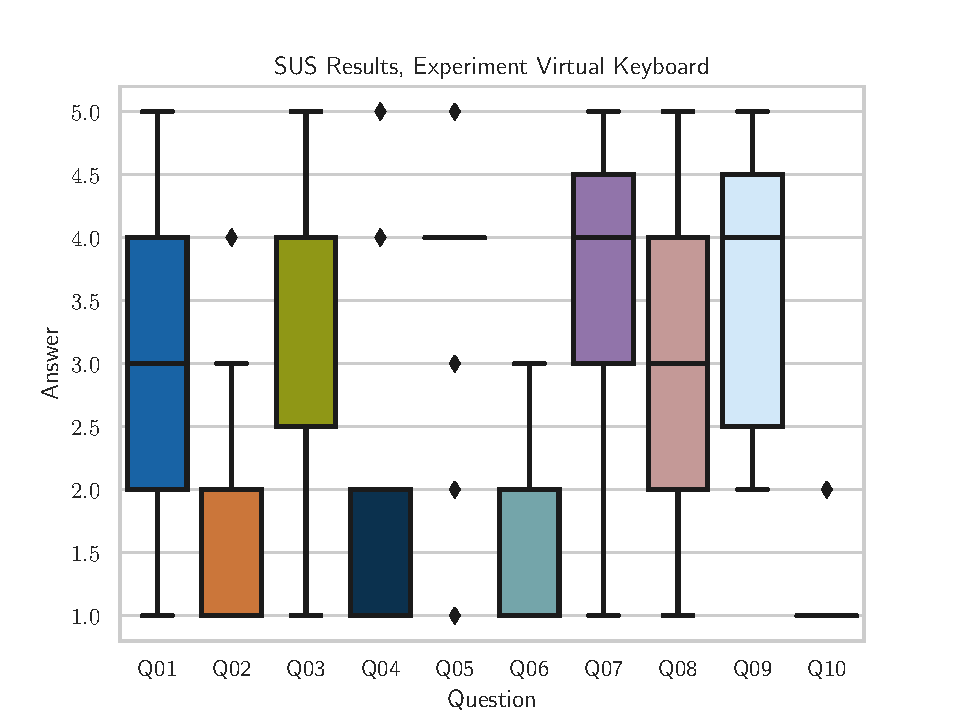
\includegraphics[width=\linewidth]{figures/evaluation/res_exp_vk.pdf}
		\caption{The results of questions one to ten.}\label{fig:res-exp-vk}
	\end{subfigure}%
	\begin{subfigure}[t]{.5\linewidth}%
		\centering
		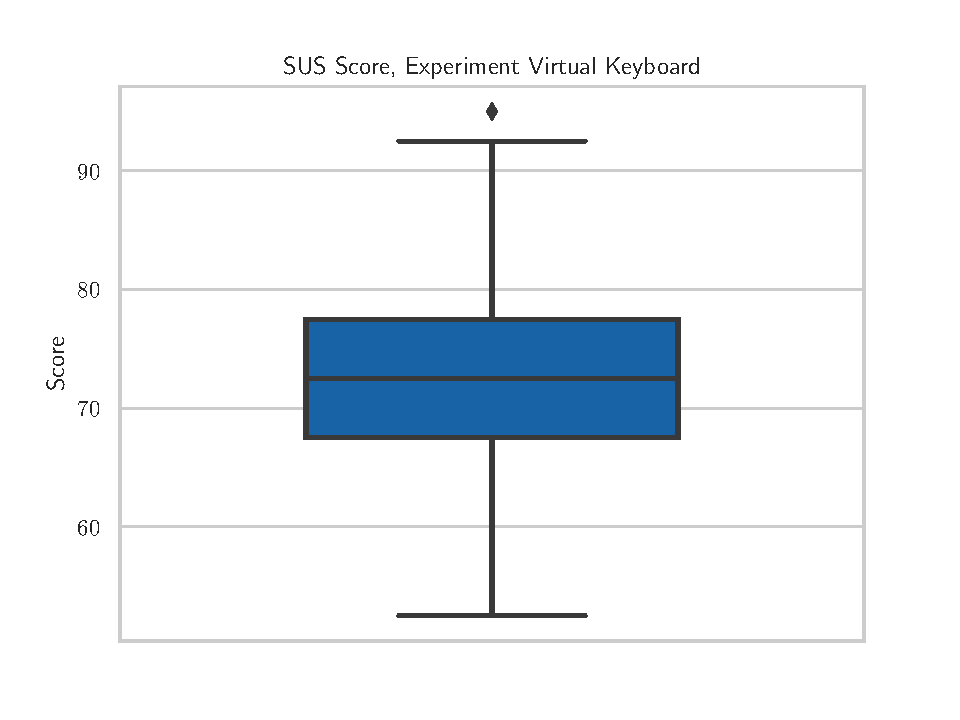
\includegraphics[width=\linewidth]{figures/evaluation/score_exp_vk.pdf}
		\caption{The overall \gls{SUS} score.}\label{fig:score-exp-vk}
	\end{subfigure}%
	\caption[Virtual keyboard SUS results]{The results of the \gls{SUS} user study for the virtual keyboard experiment.}\label{fig:exp-vk-stats}
\end{figure}

Further, many users made comments on the experiment:
\begin{itemize}
	\item The sensitivity of the movement detection should be decreased.
	\item A faster selection speed would improve comfort and typing speed.
	\item Visual, audible or haptic feedback after typing a character would be great.
	\item The one to one mapping of the display to the virtual keyboard is not very intuitive.
	\item In the input text, a caret should be displayed to visualize spaces. Also, arrow keys to navigate through the text would be handy.
	\item To improve usability, select a key instantly when the finger releases the touch screen instead of when the finger does not move for some time.
	\item It should be possible to use multiple fingers at the same time.
	\item An implementation like the Swift-keyboard for Android might be a better one, since holding the finger down was cumbersome.
	\item Another approach would be to paint characters on the screen using the touch screen or the laser pointer.
\end{itemize}
